Il paradosso di Zenone dice che per percorrere una distanza finita si devono percorrere infinite distanze finite. Ma si risolve subito: infiniti sottointervalli \emph{si possono sommare}. A volte con un risultato finito.
\[
\sum_{n = 1}^{\infty} \frac{1}{2^n} = \frac{1}{2} + \frac{1}{4} + \frac{1}{8} + \ldots = 1
\]
Le serie sono somme di successioni. Quando vogliamo calcolare una serie, vogliamo trovare questo:
\[
\sum_{n = 0}^{\infty} a_n
\]
Possiamo ricondurci a questo limite, in maniera simile a come abbiamo fatto con gli integrali impropri:
\[
\sum_{n = 0}^{\infty} a_n =
\lim_{N \to \infty} \sum_{n = 0}^{N} a_n
\]
\`E pi\`u complicato sommare un certo numero di addendi, che andare a calcolare un integrale. Nel secondo caso abbiamo il teorema fondamentale del calcolo integrale, che ci rende facile calcolare questo integrale improprio:
\[
\int_{0}^{\infty} \frac{\diff x}{1 + x^2} = \lim_{b \to \infty} \int_{0}^{b} \frac{\diff x}{1 + x^2}
\]
Mentre questa somma non \`e altrettanto facile:
\[
\sum_{n = 0}^{\infty} \frac{1}{1 + n^2}
\]

\section{Serie note}

\subsection{Serie geometrica}

L'unica serie che si sa calcolare a colpo sicuro \`e la \emph{serie geometrica}. 
\begin{defn}[Serie geometrica]
La serie geometrica \`e:
\[
\sum_{n = 0}^{\infty} \rho^n
\]
La serie vale:
\[
\sum_{n = 0}^{\infty} \rho^n = 
\frac{1}{1 - \rho}
\]
A patto che $-1 < \rho < 1$.
\end{defn}

Troviamo il suo valore. Sviluppiamola, per un certo $N$:
\begin{align*}
\sum_{n = 0}^{N} \rho^n &=
1 + \rho + \rho^2 + \rho^3 + \ldots + \rho^N = \tag{moltiplicando e dividendo per $(1 - \rho)$} \\
&= \frac{(1 + \rho + \rho^2 + \rho^3 + \ldots + \rho^N) \cdot (1 - \rho)}{1 - \rho} = \tag{sviluppando} \\
&= \frac{1 - \cancel{\rho} + \cancel{\rho} - \cancel{\rho^2} + \cancel{\rho^2} - \cancel{\rho^3} + \ldots - \cancel{\rho^{N}} + \cancel{\rho^{N}} - \rho^{N+1}}{1 - \rho} =
\frac{1 - \rho^{N+1}}{1 - \rho}
\end{align*}
Facendo ora tendere $N$ all'infinito, per $-1 < \rho < 1$:
\[
\lim_{N \to \infty} \frac{1 - \rho^{N + 1}}{1 - \rho} = \frac{1}{1 - \rho}
\]
Prendendo $\rho = \frac{1}{2}$, la serie geometrica tende a 2.

Se la serie geometrica non parte da 0, ma da un certo $n_0$, il valore della serie cambia:
\[
\sum_{n = n_0}^{\infty} \rho^n = 
\sum_{n = 0}^{\infty} \rho^{n+n_0} =
\rho^{n_0} \cdot \sum_{n = 0}^{\infty} \rho^n = \frac{\rho^{n_0}}{1 - \rho}
\]
In generale, con una serie che assomiglia a una serie geometrica, ma che non ha esattamente la forma $\sum_{n = 0}^{\infty} \rho^n$, si ``porta fuori'' dal segno di serie quello che non dipende dalla $n$.
\begin{exmp}
Consideriamo questa serie:
\[
\sum_{n = 13}^{\infty} \frac{5}{10^{3 \, n}}
\]
Il 5 si pu\`o tirar fuori.
\[
\sum_{n = 13}^{\infty} \frac{5}{10^{3 \, n}} =
5 \, \sum_{n = 13}^{\infty} \frac{1}{10^{3 \, n}}
\]
Poi, sfruttando le propriet\`a delle potenze, vediamo che $10^{3 \, n} = {\left( 10^{3} \right)}^{n}$, e quindi:
\[
5 \, \sum_{n = 13}^{\infty} \frac{1}{10^{3 \, n}} =
5 \, \sum_{n = 13}^{\infty} {\left( \frac{1}{10^3} \right)}^{n}
\]
Ora basta cambiare l'indice di partenza, e otteniamo una costante moltiplicata per una serie geometrica.
\[
\frac{5}{10^{39}} \cdot \sum_{n = 0}^{\infty} {\left( \frac{1}{10^3} \right)}^{n}
\]
\end{exmp}
Una curiosit\`a. Questa serie diverge:
\[
\sum_{n = 0}^{\infty} \sqrt{3^n}
\]
Se usassimo la formula vista prima, avremmo che:
\[
\sum_{n = 0}^{\infty} \sqrt{3^n} =
\frac{1}{1 - \sqrt{3}}
\]
Ma questo \`e un numero negativo! Una somma di infiniti numeri \emph{positivi} che d\`a un numero negativo? Assurdo! E infatti stiamo sbagliando: la serie diverge all'infinito.

\subsection{Serie telescopica}

Un'altra serie per cui sappiamo calcolare la somma \`e questa, e tutte le sue parenti.
\begin{defn}[Serie telescopica]
La serie telescopica \`e:
\[
\sum_{n = 1}^{\infty} \frac{1}{n \, (n + 1)}
\]
\end{defn}

Facciamo un'analogia: quando si studiano gli integrali di funzioni razionali, del tipo:
\[
\int \frac{\diff x}{x \, (x + 1)}
\]
Quello che facciamo \`e dividere l'integrale in una somma di due integrali.
\[
\int \frac{\diff x}{x \, (x + 1)} = \int \frac{A \dx}{x} + \int \frac{B \dx}{x + 1}
\]
In questo caso, vale che $A = 1$ e che $B = -1$. Quindi questa serie potremmo spezzarla cos\`i:
\[
\sum_{n = 1}^{\infty} \frac{1}{n \, (n + 1)} = 
\sum_{n = 1}^{\infty} \frac{1}{n} - \frac{1}{n+1}
\]
Proviamo a vedere quanto vale...
\[
\sum_{n = 1}^{\infty} \frac{1}{n} - \frac{1}{n+1} =
1 - \cancel{\frac{1}{2}} + \cancel{\frac{1}{2}} - \cancel{\frac{1}{3}} + \cancel{\frac{1}{3}} - \cancel{\frac{1}{4}} + \ldots = 1
\]
Wow.

\subsection{Serie armonica generalizzata}

Abbiamo studiato, fra gli integrali definiti, questo integrale improprio:
\[
\int_{1}^{\infty} \frac{\diff x}{x^p} = 
\begin{cases}
\text{converge per } p > 1 \\
\text{diverge per } p \le 1
\end{cases}
\]
Esiste una serie che si comporta esattamente come questo integrale improprio, ed \`e:
\[
\sum_{n = 1}^{\infty} \frac{1}{n^p} =
\begin{cases}
\text{converge per } p > 1 \\
\text{diverge per } p \le 1
\end{cases}
\]
\begin{defn}[Serie armonica generalizzata]
La serie $\sum \frac{1}{n^p}$ si chiama \emph{serie armonica generalizzata}.
\end{defn}

Grazie al \emph{criterio di convergenza integrale delle serie} (sez. \ref{sec:criterio_convergenza_integrale}) possiamo confrontare serie e integrali impropri, e dimostrare che la serie armonica generalizzata converge e diverge esattamente come l'integrale improprio $\int_{1}^{\infty} \frac{\diff x}{x^p}$.

Dall'integrale improprio di cui sopra possiamo derivare questa regola:
\[
\int_{1}^{\infty} f(x) \dx = 
\begin{cases}
\text{converge se } 0 \le f(x) \le \frac{1}{x^p} \text{ per un } p > 1 \\
\text{diverge se } f(x) \ge \frac{1}{x^p} \text{ per un } p \le 1
\end{cases}
\]
La regola analoga per le serie sar\`a:
\[
\sum_{n = 1}^{\infty} a_n =
\begin{cases}
\text{converge se } 0 \le a_n \le \frac{1}{n^p} \text{ per un } p > 1 \\
\text{diverge se } a_n \ge \frac{1}{n^p} \text{ per un } p \le 1
\end{cases}
\]

\section{Determinare la convergenza di una serie} 

Consideriamo questa serie:
\begin{equation} \label{eq:serie_non_convergente}
\sum_{n = 0}^{\infty} \frac{n}{n + 2}
\end{equation}
Converge? A cosa? Possiamo vedere che vale questo, studiando la successione associata alla serie:
\[
\lim_{n \to \infty} \frac{n}{n+2} = 1
\]
Pu\`o la somma di infiniti termini che tendono a 1, tendere a qualcosa di finito? Intuitivamente no. E infatti fra poco lo formalizzeremo...

\subsection{Criterio del confronto}

Consideriamo due generiche serie:
\[
\sum_{n = n_0}^{\infty} a_n \qquad
\sum_{n = n_0}^{\infty} b_n
\]
Supponiamo valga, fra le successioni $a_n$ e $b_n$, una disuguaglianza del tipo $0 \le a_n \le b_n$, $\forall n \ge n_0$. Possiamo dire che vale, quindi, questo:
\[
\sum_{n = n_0}^{\infty} a_n \le
\sum_{n = n_0}^{\infty} b_n
\]
Consideriamo la successione $S_N$ definita a partire dalla prima serie.
\[
S_N = \sum_{n = n_0}^{N} a_n
\]
Possiamo vedere che questa successione \`e crescente. Le successioni monotone e limitate convergono, quelle monotone e \emph{non} limitate divergono. Si dice che le successioni monotone sono \emph{regolari}, ossia o divergono -positivamente o negativamente- o convergono.

Facciamo un'analogia con gli integrali. Consideriamo una funzione $f(x) \ge 0$, e l'integrale generico:
\[
F(k) = \int_{1}^{k} f(x) \dx
\]
La funzione $F(k)$ \`e una funzione crescente. Il limite $\lim_{k \to \infty} F(k)$ converge o diverge positivamente, proprio come succede con le successioni.

Quello che abbiamo visto confrontando gli integrali impropri di funzioni tipo $f(x) \le g(x)$, \`e simile a quanto vale con il confronto fra serie. Se l'integrale improprio $\int_{1}^{\infty} g(x)$ converge, anche l'integrale improprio $\int_{1}^{\infty} f(x)$ converge.

Ricapitolando, se vale che $0 \le a_n \le b_n$, sappiamo che entrambe le serie sono regolari, quindi o divergono positivamente o convergono.

Ma possiamo dire di pi\`u:
\[
\sum_{n = n_0}^{\infty} a_n \le
\sum_{n = n_0}^{\infty} b_n
\]
Se la prima serie diverge, anche la seconda diverge. Se la seconda serie converge, anche la prima converge.

Per dimostrare che la serie nell'equazione \ref{eq:serie_non_convergente} diverge, possiamo dire che:
\[
\frac{n}{n+2} \ge \frac{1}{2} \text{ per } n \ge 2
\]
Quindi, per quanto appena visto:
\[
\sum_{n = 2}^{\infty} \frac{n}{n+2} \ge \sum_{n = 2}^{\infty} \frac{1}{2}
\]
E la seconda serie diverge! Quindi, essendo la prima maggiore di qualcosa che diverge, diverge anch'essa.

La successione $a_n = \frac{1}{2}$ \`e una \emph{successione costante}.

\begin{exmp}
La convergenza di questa serie si determina per confronto:
\[
\sum_{n = 1}^{\infty} \frac{1 + n!}{(1 + n)!}
\]
I termini della serie si possono esprimere cos\`i:
\[
\frac{1 + n!}{(1 + n)!} = \frac{1}{(1 + n)!} + \frac{n!}{(1 + n)!} = \frac{1}{(1 + n)!} + \frac{1}{1 + n}
\]
La serie del primo termine \`e convergente:
\[
\sum_{n = 1}^{\infty} \frac{1}{(1 + n)!} \le \sum_{n = 1}^{\infty} \frac{1}{n \, (n + 1)}
\]
La serie del secondo termine non lo \`e, comportandosi come $\frac{1}{n}$. \`E sufficiente ricordarsi che la serie delle somme \`e la somma delle serie.
\end{exmp}

\subsubsection{Criteri del confronto fra integrali e serie}

Possiamo accomunare la convergenza delle serie e la convergenza degli integrali perch\'e entrambi i problemi sfruttano il teorema del confronto, in molti casi, per trovare una risposta.

Data una funzione $f(x)$ tale che $0 \le g(x) \le f(x) \le h(x)$, vale che:
\[
0 \le \int_{a}^{\infty} g(x) \dx \le \int_{a}^{\infty} f(x) \dx \le \int_{a}^{\infty} h(x) \dx
\]
Ora, considerando due funzioni $f(x)$ e $g(x)$, entrambe ``problematiche'' in un certo $x_0$, se vale questo:
\[
\lim_{x \to x_0} \frac{f(x)}{g(x)} = L \in \ooint{0}{\infty}
\]
significa che $f(x) \sim g(x)$, ossia che vale questa disuguaglianza:
\[
\frac{1 \, L}{2} \cdot g(x) \le f(x) \le \frac{3 \, L}{2} \cdot g(x)
\]
Lo stesso ragionamento \`e applicabile alle serie (considerando per ora solo serie a termini positivi).

Se abbiamo tre successioni tali che $0 \le c_n \le a_n \le b_n$, allora vale questo:
\[
0 \le \sum_{n} c_n \le \sum_{n} a_n \le \sum_{n} b_n 
\]
Se $c_n$ diverge, diverge anche $a_n$, se invece $b_n$ converge, converge anche $a_n$.

Con le serie, il criterio asintotico diventa questo:
\[
\lim \frac{a_n}{b_n} = L \in \ooint{0}{\infty}
\]
Questo vuol dire che $a_n \sim b_n$, ossia $a_n$ si comporta \emph{asinotitcamente} come $b_n$, ossia vuol dire che (per un $N$ sufficientemente grande!) vale questo:
\[
\frac{1 \, L}{2} \cdot b_n \le a_n \le \frac{3 \, L}{2} \cdot b_n
\]
Ossia, la convergenza (o divergenza) di $a_n$ dipende dalla convergenza (o divergenza) di $b_n$.

Nel caso delle serie, tutto sta nel trovare delle (altre) serie di cui gi\`a sappiamo convergenza o divergenza con cui fare il confronto.

Tipicamente, si prendono i termini pi\`u importanti del numeratore e del numeratore, si fa il rapporto fra i due e si trova quindi la serie con cui fare il confronto.

\subsection{Condizione necessaria per la convergenza}

All'inizio della sezione precedente, abbiamo promesso di formalizzare qualcosa di intuitivo.
\begin{theorem}
Condizione necessaria affinch\'e la somma di $a_n$ converga \`e che la successione $a_n$ converga (o tenda) a 0.
\end{theorem}
Perch\'e \`e una \emph{condizione necessaria}? Considerando la somma parziale della serie:
\[
S_N = \sum_{n = 0}^{N} a_n
\]
Vale che $S_N = S_{N - 1} + a_n$. Se la serie converge, sia $S_N$ che $S_{N - 1}$ tendono a una certa quantit\`a $L \in \reals$. Quindi, necessariamente, $a_n$ deve tendere a 0.

\subsection{Criterio di convergenza integrale}
\label{sec:criterio_convergenza_integrale}

Consideriamo una successione $a_n$ e una funzione $f(x)$ per cui vale:
\begin{align*}
f(N_0 + 1) &= a_{N_0 + 1} \\
f(N_0 + 2) &= a_{N_0 + 2} \\
\ldots 
\end{align*}
Nella figura \ref{fig:integrale_maggiora_serie}, la somma dei rettangoli (larghi 1 e alti quanto $a_n$) \`e minore dell'integrale della funzione.

\begin{figure}
\centering
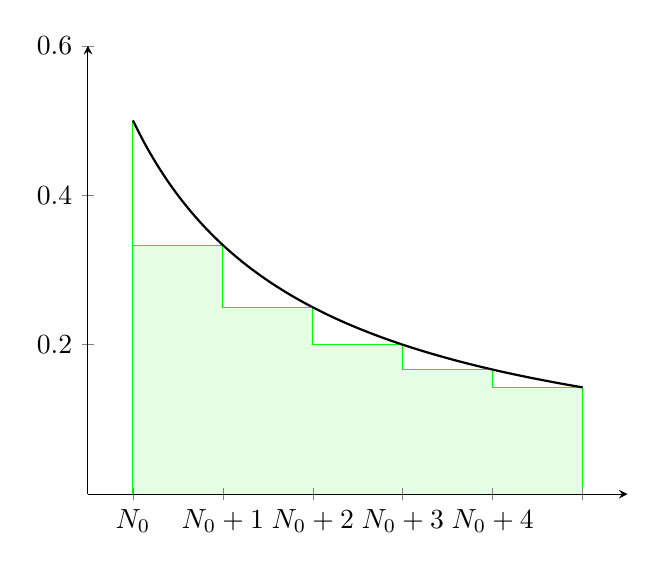
\begin{tikzpicture}[scale=1.0]
\begin{axis}[
    % xtick={0,...,1.5},ytick={0,...,1.5},
    % xmax=2,ymax=1.2,ymin=0,xmin=0,
    % enlargelimits=true,
    xticklabels={$N_0$,$N_0$,$N_0$,$N_0 + 1$,$N_0 + 2$,$N_0 + 3$,$N_0 + 4$},
    axis lines=middle,
    clip=false,
    ymax=0.6,
    ymin=0,
    xmin=1.5,
    xmax=7.5,
    domain=2:7,
    axis on top
    ]

\addplot [draw=green, fill=green!10, const plot mark right, samples=6, domain=2:7]
    {1 / x}\closedcycle;

\addplot[smooth, thick,domain=2:7,samples=40]{1 / x};

\end{axis}
\end{tikzpicture}
\caption{\label{fig:integrale_maggiora_serie}L'integrale della funzione maggiora la serie}
\end{figure}

La serie \`e la somma delle aree dei rettangoli, mentre l'integrale \`e l'area sotto la curva. Vale evidentemente che:
\[
\sum_{n \ge N_0 + 1}^{\infty} a_n \le \int_{N_0 + 1}^{\infty} f(x) \dx
\]
Quindi, se l'integrale improprio converge, converge anche la serie.

Usiamo questa propriet\`a per studiare la convergenza delle serie armoniche generalizzate, come questa:
\[
\sum_{n = 1}^{\infty} \frac{1}{n^2} \le \int_{1}^{\infty} \frac{\diff x}{x^2} < \infty
\]
Il ragionamento alla base di questi confronti \`e propriamente geometrico. 

Quindi, nel caso generale, vale questo:
\[
\sum_{n = 1}^{\infty} \frac{1}{n^p} \le \int_{1}^{\infty} \frac{\diff x}{x^p} < \infty \text{ per } p > 1
\]

Come facciamo vedere, ora, che la serie diverge per $p \le 1$? Vogliamo scrivere che la sommatoria sia maggiore o uguale all'integrale, quindi dobbiamo costruire il grafico (e di conseguenza la funzione) in modo che i rettangoli della serie contengano il grafico della funzione.

\begin{figure}
\centering
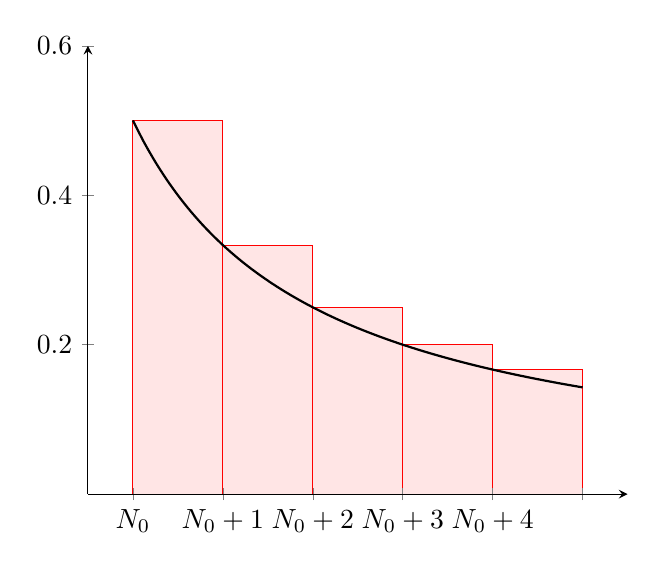
\begin{tikzpicture}[scale=1.0]
\begin{axis}[
    % xtick={0,...,1.5},ytick={0,...,1.5},
    % xmax=2,ymax=1.2,ymin=0,xmin=0,
    % enlargelimits=true,
    xticklabels={$N_0$,$N_0$,$N_0$,$N_0 + 1$,$N_0 + 2$,$N_0 + 3$,$N_0 + 4$},
    axis lines=middle,
    clip=false,
    ymax=0.6,
    ymin=0,
    xmin=1.5,
    xmax=7.5,
    domain=2:7,
    axis on top
    ]

\addplot [draw=red, fill=red!10, ybar interval, samples=6, domain=2:7]
    {1 / x}\closedcycle;

\addplot[smooth, thick,domain=2:7,samples=40]{1 / x};
\end{axis}
\end{tikzpicture}
\caption{\label{fig:serie_maggiora_integrale}La serie maggiora l'integrale della funzione}
\end{figure}

La disuguaglianza che ci interessa ora:
\[
\int_{N_0 + 1}^{\infty} f(x) \dx \le \sum_{n \ge N_0}^{\infty} a_n 
\]

Quindi, alla fine, il sottografico della funzione $f(x)$ (nella figura \ref{fig:serie_maggiora_integrale}) \`e compreso fra le due serie:
\[
\sum_{n \ge N_0 + 1}^{\infty} a_n \le
\int_{N_0 + 1}^{\infty} f(x) \dx \le 
\sum_{n \ge N_0}^{\infty} a_n 
\]
Cambia il punto di partenza delle serie (una parte da $N_0$, l'altra da $N_0 + 1$).

Ai fini pratici, ci interessa il fatto che vale questa disuguaglianza:
\[
\int_{N_0 + 1}^{\infty} f(x) \dx \le 
\sum_{n = N_0}^{\infty} a_n \le
\int_{N_0}^{\infty} f(x) \dx
\]

\begin{exmp}[di applicazione del criterio integrale]
Questa serie \`e impossibile da maggiorare o da minorare:
\[
\sum_{n = 2}^{\infty} \frac{1}{n \, \log (n) \, {\left[ \log \left( \log (n) \right) \right]}^{2}}
\]
Funziona per\`o il criterio integrale, che ci mostra che l'integrale converge:
\[
\int_{2}^{\infty} \frac{\diff x}{x \, \log(x) \, {\left[ \log \left( \log (x) \right) \right]}^{2}} = \increment{- \frac{1}{\log \left( \log(x) \right)}}^{\infty}_{2} = \frac{1}{\log \left( \log(2) \right)}
\]
Osservando la serie iniziale, e pensando all'integrale che le si pu\`o associare, si nota la presenza di una funzione e della sua derivata:
\[
\frac{1}{f'(x) \, {\left[ f(x) \right]}^2}
\]
Con $f(x) = \log \left( \log(x) \right)$, e quindi $f'(x) = \frac{1}{x \, log \left( x \right)}$.
\end{exmp}

\subsection{Criterio asintotico}

Il criterio asintotico permette di determinare la convergenza o divergenza di una serie studiando il comportamento al limite delle successioni loro associate.

Supponiamo di avere due successioni $a_n$ e $b_n$, e che valga questo:
\[
\lim_{n \to \infty} \frac{a_n}{b_n} = L \in \ooint{0}{\infty}
\]
Per un $n$ approriato, varr\`a che:
\[
\frac{L}{2} \le \frac{a_n}{b_n} \le \frac{3 \, L}{2}
\implies
\frac{L \, b_n}{2} \le a_n \le \frac{3 \, L \, b_n}{2}
\]
Quindi, se la serie di $b_n$ diverge, diverger\`a anche la serie di $a_n$, e se la serie di $b_n$ converge, converger\`a anche la serie di $a_n$.

\begin{exmp}
Consideriamo questa serie:
\[
\sum_{n = 1}^{\infty} \frac{1}{n^3 + 2 \, n - \sqrt{n} + 24}
\]
Non viene facile una maggiorazione o una minorazione: al denominatore c'\`e un $- \sqrt{n}$ che non \`e ben chiaro cosa fa. Per\`o, abbiamo il criterio del confronto asintotico per determinare la convergenza della serie. Facciamo quindi il limite del rapporto con $b_n = \frac{1}{n^3}$:
\[
\lim_{n \to \infty} \frac{n^3}{n^3 + 2 \, n - \sqrt{n} + 24} = 1
\]
Quindi, siccome questa serie converge:
\[
\sum_{n = 1}^{\infty} \frac{1}{n^3}
\]
converge anche la serie all'inizio.
\end{exmp}

\subsection{Criterio del rapporto}

Consideriamo una serie $\sum_{n} a_n$, tale per cui $a_n \ge 0$. Per verificare la convergenza o la divergenza della serie si pu\`o usare il criterio del rapporto:
\[
\lim_{n \to \infty} \frac{a_{n+1}}{a_n} = 
\begin{cases}
L < 1 \implies \sum_{n} a_n \text{ converge} \\
L > 1 \implies \sum_{n} a_n \text{ diverge} \\
1 \implies \text{ non si pu\`o dire nulla su } \sum_{n} a_n
\end{cases}
\]
Stiamo vedendo a cosa tende il rapporto fra il termine e il termine che lo precede.

\begin{exmp}
Consideriamo la serie:
\[
\sum_{n = 1}^{\infty} \frac{e^n}{n!}
\]
Applichiamo il criterio del rapporto:
\[
\lim_{n \to \infty} \frac{e^{n+1}}{(n+1)!} \cdot \frac{n!}{e^n} = 
\lim_{n \to \infty} \frac{e}{n+1} = 0
\]
Quindi la serie converge.
\end{exmp}

\subsection{Criterio della radice}

\[
\lim_{n \to \infty} \sqrt[n]{a_n} = 
\begin{cases}
L < 1 \implies \sum_{n} a_n \text{ converge} \\
L > 1 \implies \sum_{n} a_n \text{ diverge} \\
1 \implies \text{ non si pu\`o dire nulla su } \sum_{n} a_n
\end{cases}
\]
Stiamo facendo il limite per $n$ che tende all'infinito della radice $n$-esima dell'$n$-esimo termine della successione.

Entrambi questi criteri si vedono confrontandoli con la serie geometrica. Sono sempre applicazioni del criterio del confronto, da cui viene fuori la serie geometrica. \`E facile vederlo col criterio della radice.

Supponiamo il limite di $\sqrt[n]{a_n}$ sia maggiore di 1. Vuol dire che $\sqrt[n]{a_n} \ge 1 \iff a_n \ge 1$ da un certo punto in poi, e quindi $a_n$ non tende a 0, e quindi necessariamente diverge.

Supponiamo di essere nel caso in cui il limite sia minore di 1. Quindi per ogni $\varepsilon > 0$ tale per cui $L + \varepsilon < 1$, risulta che:
\[
\sqrt[n]{a_n} \le L + \varepsilon \le 1
\]
Questo equivale a dire, elevando entrambi i membri alla potenza $n$, che:
\[
a_n \le \left( L + \varepsilon \right)^{n}
\]
$L + \varepsilon$ \`e minore di 1, quindi la serie geometrica che gli associamo converge:
\[
\sum_{n = 1}^{\infty} \left( L + \varepsilon \right)^{n} \le \infty
\]
Ci siamo procurati una maggiorazione con una serie geometrica dal calcolo della radice $n$-esima di $a_n$.

Con il criterio del rapporto, invece, il ragionamento \`e questo:
\[
\frac{a_{n+1}}{a_n} \le L + \epsilon \iff a_{n+1} \le \left( L + \varepsilon \right) \cdot a_n
\]
Analogamente, valgono queste disuguaglianze:
\begin{align*}
a_{n+2} \le \left( L + \varepsilon \right) \cdot a_{n + 1} \le
\left( L + \varepsilon \right)^2 \cdot a_{n} \\
a_{n+3} \le \left( L + \varepsilon \right)^3 \cdot a_{n}
\end{align*}
E quindi ci esce di nuovo fuori una serie geometrica...

Come mai nessuno dei criteri vale quando il limite tende a 1? Boh.

% TODO riempire

\section{Serie a termini non tutti positivi}

Se non \`e vero che $a_n \ge 0$ per ogni $n$, quanto detto per il criterio del confronto non \`e pi\`u valido.

Tutti i ragionamenti fatti fino ad ora sono stati fatti con serie a termini non negativi. Cosa succede se i termini sono \emph{anche} negativi?

Se la serie \`e (anche) a termini negativi, studiamo la serie dei moduli:
\[
\sum_{n}^{\infty} \abs{a_n}
\]
\begin{defn}
Se la serie di $\abs{a_n}$ converge, si dice che la serie di $a_n$ converge \emph{assolutamente}.

Ossia, se la serie dei moduli converge, converge anche la serie di partenza. Non vale il viceversa.
\end{defn}

Supponiamo di avere una serie a termini $a_n$ anche negativi. Consideriamo la successione:
\[
b_n = a_n + \abs{a_n}
\]
Vale ovviamente che $b_n \ge 0$. Infatti, se $a_n < 0$, $a_n + \abs{a_n} = 0$, altrimenti $a_n + \abs{a_n} = 2 \, a_n \ge 0$.

Quindi $b_n \le 2 \, \abs{a_n}$. Se converge $\abs{a_n}$, converge anche $b_n$. Quindi, essendo $a_n = b_n - \abs{a_n}$, vuol dire che la serie $a_n$ converge.

Se il criterio del rapporto e il criterio della radice non funzionano, tipicamente significa che \`e necessario trovare una serie con cui fare un confronto.

\subsection{Criterio di Leibniz}

Introduciamo il criterio di Leibniz per somma di successioni a termini di segni alterno. 

\begin{theorem}[Criterio di Leibniz]
Se le seguenti ipotesi sono vere:
\begin{enumerate}
    \item $a_n \cdot a_{n+1} \le 0 \forall n$, ossia ogni termine ha segno opposto rispetto al successivo. Quindi la serie sar\`a qualcosa del tipo:
    \[
    \sum_{n} a_n = \sum_{n} (-1)^n \alpha_n
    \]
    Con $\alpha_n \ge 0$, e in particolare $\alpha_n = \abs{a_n}$.
    \item $\abs{a_{n+1}} \le \abs{a_n}$, ossia $\alpha_{n+1} \le \alpha_{n}$, ossia il valore assoluto dei termini non cresce.
    \item $\lim_{n \to \infty} a_n = 0$, ossia la successione associata alla serie tende a 0.
\end{enumerate}
allora la serie di $a_n$ converge.
\end{theorem}

\begin{proof}[del criterio di Leibniz]
Abbiamo una successione $a_n$ e, per ipotesi:
\begin{enumerate}
    \item $lim_{n \to \infty} a_n = 0$
    \item $a_n \cdot a_{n+1} < 0$
    \item $\abs{a_n} \ge \abs{a_{n+1}}$
\end{enumerate}
Senza perdita di generalit\`a, assumiamo valga $a_{2 \, n + 1} > 0$ e $a_{2 \, n} < 0$.

La serie $S_{2 \, n}$ dei termini pari \`e monotona crescente:
\[
S_{2 \, (n + 1)} = S_{2 \, n} + a_{2 \, n + 1} + a_{2 \, n + 2}
\]
Vale infatti che $a_{2 \, n + 1} > 0$ e che $a_{2 \, n + 2} < 0$, e che $\abs{a_{2 \, n + 1}} \ge \abs{a_{2 \, n + 2}}$, da cui segue che $a_{2 \, n + 1} + a_{2 \, n + 2} \ge 0$. Allo stesso modo, la serie $S_{2 \, n + 1}$ dei termini dispari \`e monotona decrescente.

Entrambe le serie sono limitate superiormente e inferiormente. Di base vale che $S_1 = a_1 > a_1 + a_2 = S_2$, e in generale che $S_{2 \, m + 1} > S_{2 \, m}$. Aggiungendoci che le serie sono una decrescente e una crescente, abbiamo che:
\[
S_1 > S_{2 \, m + 1} > S_{2 \, m} > S_2
\]
La serie dei termini dispari \`e monotona decrescente e limitata inferiormente, la serie dei termini pari \`e monotna crescente e limitata superiormente. Entrambe convergono.

Per concludere la dimostrazione, dimostriamo che convergono allo stesso valore. Infatti:
\[
\lim_{n \to \infty} S_{2 \, n + 1} - S_{2 \, n} = 
\lim_{n \to \infty} a_{2 \, n + 1} = 0
\]
La loro differenza tende a 0, quindi convergono entrambe allo stesso valore.
\end{proof}

Consideriamo questa serie:
\[
\sum_{n = 1}^{\infty} (-1)^n \frac{1}{n^p} \qquad \text{con } p \ge 0
\]
Per $p \ge 1$, sappiamo gi\`a che la serie dei moduli converge, e che quindi questa serie converge assolutamente. Ma, grazie al criterio di Leibniz, sappiamo che la serie converge anche per $0 < p \le 1$.

\subsection{Riordinare le serie}

Con serie a termini tutti positivi o tutti negativi, i termini possono essere riordinati senza problemi: si pu\`o ``commutare l'ordine degli addendi'', senza cambiare la convergenza o divergenza della serie, n\'e il valore a cui converge. Riemann dimostr\`o che non si pu\`o sempre fare lo stesso con serie a termini di segno differente.

Consideriamo questa serie:
\[
\sum_{n = 1}^{\infty} \frac{(-1)^n}{\sqrt{n}}
\]
Sommiamo prima i termini pari, fino a un certo termine $a_p$, tale per cui la somma fino a $p$ \`e maggiore di un certo numero, ad esempio $\frac{3}{4}$.
\[
\frac{1}{\sqrt{2}} + \frac{1}{\sqrt{4}} + \frac{1}{\sqrt{6}} + \ldots + \frac{1}{\sqrt{2 \, p}} > \frac{3}{4}
\]
Ora aggiungiamo i termini dispari, fino a quando la somma dei termini pari e dei termini dispari non diventa minore di $\frac{3}{4}$.
\[
\frac{1}{\sqrt{2}} + \frac{1}{\sqrt{4}} + \frac{1}{\sqrt{6}} + \ldots + \frac{1}{\sqrt{2 \, p}} - \frac{1}{\sqrt{3}} - \frac{1}{\sqrt{5}} - \frac{1}{\sqrt{7}} - \ldots - \frac{1}{\sqrt{2 \, p + 1}} < \frac{3}{4}
\]
Continuando a sommare i termini in questo modo, il risultato finale della serie riordinata sar\`a $\frac{3}{4}$: sommando i termini nel modo che abbiamo indicato, infatti, la serie \emph{tende a $\frac{3}{4}$}.

\subsubsection{Riordinare serie convergenti assolutamente}

Consideriamo una serie con termini a segno alterno:
\[
\sum_{n = 1}^{\infty} a_n \text{ t.c. } a_{2 \, k + 1} \ge 0 \land a_{2 \, k} \le 0 \forall k \in \naturals
\]
Se $\sum a_n$ converge assolutamente, allora devono convergere sia la serie dei termini dispari $\sum a_{2 \, k + 1}$, sia la serie dei termini pari $\sum a_{2 \, k}$.

Vale infatti questa disuguaglianza:
\[
\sum_{k = 1}^{N} a_{2 \, k - 1} \le \sum_{n = 1}^{2 \, N -1} \abs{a_n}
\]
Espandendola per $N = 2$, abbiamo:
\[
a_1 + a_3 \le \abs{a_1} + \abs{a_2} + \abs{a_3}
\]
La somma dei termini positivi \`e maggiorata dalla somma dei moduli di tutti i termini. Quindi vale questo, in generale:
\[
\sum_{k = 1}^{N} a_{2 \, k - 1} \le \sum_{n = 1}^{2 \, N -1} \abs{a_n}
\le \sum_{n = 1}^{\infty} \abs{a_n} < \infty
\]
Se la serie converge assolutamente, converge anche la serie dei termini positivi, poich\'e quest'ultima \`e maggiorata dalla serie dei moduli.

I termini di indice pari, invece, sono tutti negativi. La disuguaglianza che vale \`e questa:
\[
\sum_{k = 1}^{N} a_{2 \, k} \ge - \sum_{n = 1}^{2 \, N} \abs{a_n}
\ge - \sum_{n = 1}^{\infty} \abs{a_n} > - \infty
\]
La serie dei termini pari \`e \emph{minorata da un numero negativo}. La serie dei termini pari \`e minore o pari a 0, e quindi il suo valore \`e necessariamente compreso fra 0 e un numero negativo \emph{diverso da $- \infty$}. Quindi converge anche la serie dei termini pari.

Se vale che le serie dei termini pari e quella dei termini dispari convergono, allora converger\`a anche la serie normale:
\[
\sum_{n = 1}^{2 \, M} a_n = \sum_{k = 1}^{M} a_{2 \, k - 1} + \sum_{k = 1}^{M} a_{2 \, k}
\]
L'equazione che abbiamo ora scritto ha \emph{riordinato} i termini. Possiamo farlo perch\'e \emph{entrambe le serie convergono}. Se non convergessero, non si potrebbero riordinare i termini.

\subsubsection{Riordinare serie convergenti semplicemente}

Questo ragionamento non vale pi\`u per serie con termini di segno alterno che convergono \emph{semplicemente}, e che quindi non convergono assolutamente.

Se la serie converge semplicemente, vuol dire che vale questo:
\[
\sum_{k} a_{2 \, k + 1} = \infty \text{ e } \sum_{k} a_{2 \, k} = - \infty
\]
Perch\'e una serie converga semplicemente, le serie dei termini pari e dispari devono tendere rispettivamente all'infinito e a meno infinito (o viceversa). Se tendesse all'infinito positivo solo una delle due (o tutte e due), la serie divergerebbe. Se nessuna delle due tendesse all'infinito, la serie convergerebbe assolutamente.

Se si riordina una serie che converge semplicemente, la si pu\`o far tendere a qualsiasi valore, perch\'e, in realt\`a, si sta creando \emph{un'altra} serie.

% END BOH

\section{Serie di potenze}

Introduciamo le serie di potenze con un esempio.

\begin{exmp}
Consideriamo questa serie:
\[
\sum_{n = 1}^{\infty} \frac{(x - 5)^n}{\sqrt{n}}
\]
Ci chiediamo: per quali valori di $x$ questa serie converge assolutamente? Per quali converge semplicemente? Per quali \emph{non} converge? Possiamo vedere che per $x = 5$, la serie \`e la serie di tutti 0, che converge. Per $x = 6$, la serie diverge.

In generale, se $x \ge 5$, la serie \`e una serie a termini positivi, e quindi possiamo applicare i criteri che abbiamo gi\`a visto. Ad esempio, si pu\`o applicare il criterio del rapporto.
\[
\lim_{n \to \infty} \frac{(x - 5)^{n+1}}{\sqrt{n+1}} \, \frac{\sqrt{n}}{(x - 5)^n} = \lim_{n \to \infty} (x - 5) \frac{\sqrt{n}}{\sqrt{n+1}} = (x - 5)
\]
Quindi il rapporto tende a $x - 5$. Se $5 < x < 6$, la serie converge, quindi sappiamo che la serie converge per $x \in \coint{5}{6}$, diverge per $x \in \coint{6}{\infty}$.

Per scoprire dove converge assolutamente, studiamo la serie:
\[
\sum_{n = 1}^{\infty} \frac{\abs{x - 5}^n}{\sqrt{n}}
\]
Applicando il criterio del rapporto a questa serie troviamo che converge per $\abs{x - 5} < 1$, e che diverge per $\abs{x - 5} > 1$.

Quindi, per $\abs{x - 5} < 1$, ossia per $4 < x < 5$, la serie converge assolutamente. Per $x$ pari a $5$, la serie diverge. Per $x$ pari a $4$, la serie converge, essendo uguale a:
\[
\sum_{n = 1}^{\infty} \frac{(-1)^n}{\sqrt{n}}
\]
Che converge (semplicemente) per il criterio di Leibniz.
\end{exmp}

Per studiare queste serie, si applica il criterio del rapporto alla serie dei moduli, per trovare gli intervalli in cui la serie converge assolutamente. Poi, si studiano i punti in cui il criterio del rapporto ha limite 1, per scoprire se la serie converge o diverge anche in quei punti.

Le serie di potenze sono serie nella forma:
\[
\sum_{n = 0}^{\infty} a_n \cdot (x - x_0)^n
\]
$x_0$ \`e chiamato ``centro''. I casi che possono verificarsi sono:
\begin{enumerate}
    \item la serie converge solo per $x = x_0$
    \item la serie converge per ogni $x$
    \item esiste un numero $R \in \ooint{0}{\infty}$ tale che la serie converge assolutamente per $\abs{x - x_0} < R$ e non converge per $\abs{x - x_0} > R$. Non diciamo niente sui casi in cui $\abs{x - x_0} = R$.
\end{enumerate}

Per verificare cosa succede, facciamo subito la sostituzione $y = x - x_0$, e riconduciamoci alla serie seguente (di centro 0):
\[
\sum_{n = 0}^{\infty} a_n \cdot y^n
\]
Studiamo la serie dei moduli, cercando per quali valori di $y$ si ha che $\abs{a_n} \cdot \abs{y}^n < \infty$.

Dobbiamo applicare il criterio del rapporto, avendo una serie a termini positivi.
\[
\lim_{n \to \infty} \frac{\abs{a_{n+1}} \cdot \abs{y}^{n+1}}{\abs{a_n} \cdot \abs{y}^n} = \frac{\abs{a_{n+1}}}{\abs{a_n}} \cdot \abs{y}
\]
Supponiamo che il limite $\frac{\abs{a_{n+1}}}{\abs{a_n}}$ tenda a un certo $L \in \ooint{0}{\infty}$. Quindi il limite del rapporto tende a $\abs{y} \cdot L$.
\begin{itemize}
    \item se $\abs{y} \cdot L < 1$, la serie converge assolutamente.
    \item se $\abs{y} \cdot L > 1$, la serie diverge.
    \item se $\abs{y} \cdot L = 1$, non sappiamo niente.
\end{itemize}

La serie converge assolutamente per $\abs{y} < \frac{1}{L}$, quindi per $\abs{x - x_0} < \frac{1}{L}$, ossia:
\[
x_0 - \frac{1}{L} < x < x_0 + \frac{1}{L}
\]
$R = \frac{1}{L}$ si chiama \emph{raggio di convergenza}.

\begin{exmp}
Consideriamo questa serie di potenze:
\[
\sum_{n = 1}^{\infty} \frac{x^n}{n^p} \forall p
\]
Il centro della serie \`e 0. Il suo raggio di convergenza \`e 1:
\[
\lim_{n \to \infty} \frac{n^p}{(n+1)^p} = 1
\]
Quindi la serie converge assolutamente per $-1 < x < 1$. Ma per $x = 1$ e per $x = -1$? Dobbiamo studiare questi casi a parte.

Per $x = 1$, la convergenza e divergenza dipende dal valore del parametro $p$.
\[
\sum_{n = 1}^{\infty} \frac{1}{n^p} < \infty \iff p > 1
\]
Per $x = -1$, la serie diventa:
\[
\sum_{n = 1}^{\infty} \frac{(-1)^n}{n^p}
\]
\`E una serie a termini di segno alterno. Se $p > 1$, la serie converge assolutamente, poich\'e la serie dei moduli \`e quella appena vista. Per $0 < p \le 1$, la serie converge semplicemente.

In sintesi, la serie converge assolutamente per $\abs{x} < 1$, non converge per $\abs{x} > 1$.

Per $x = 1$, la serie converge $\iff p > 1$.

Per $x = -1$, la serie converge assolutamente se $p > 1$, converge semplicemente se $0 < p \le 1$.
\end{exmp}

\subsection{Serie di potenze, derivate, e integrali}

Consideriamo una generica serie di potenze:
\[
\sum_{n = 0}^{\infty} a_n \, (x - x_0)^n
\]
con raggio di convergenza $R \in \ocint{0}{\infty}$. Vuol dire che la serie converge per $- R < x - x_0 < R$.

Possiamo vedere questa serie come una funzione $f(x)$, definita per $\abs{x - x_0} < R$, ossia per $x \in \ooint{x_0 - R}{x_0 + R}$ (che \`e chiamato \emph{intervallo di convergenza}). 
\[
f(x) = \sum_{n = 0}^{\infty} a_n \, (x - x_0)^n
\]
Questa funzione \`e derivabile, e la sua derivata \`e la somma delle derivate:
\[
f'(x) = \sum_{n = 1}^{\infty} n \, a_{n} \, (x - x_0)^{n - 1}
\]
E non solo: essendo derivabile, questa funzione \`e anche integrabile:
\[
\int_{x_0}^{x} f(x) \dx = 
\sum_{n = 0}^{\infty} \int_{x_0}^{x} a_n \, (x - x_0)^n =
\sum_{n = 0}^{\infty} a_n \, \frac{(x - x_0)^{n + 1}}{n + 1}
\]
Le serie di potenze sono integrabili e derivabili termine a termine \emph{all'interno dell'intervallo di convergenza}. E il discorso, poi, vale anche per la derivata della derivata, e per la derivata della derivata della derivata... La derivata $k$-esima \`e:
\[
f^{(k)} (x) = \sum_{n = k} n \cdot (n - 1) \cdot \ldots \cdot (n - k + 1) \, a_n \, (x - x_0)^{n - k}
\]
Dicendo che $0^0 = 1$ (\`e un abuso di notazione, ma a noi va bene), vediamo quanto vale la funzione (e le sue derivate) in $x = x_0$:
\begin{align*}
f(x_0) &= a_0 \\
f'(x_0) &= a_1 \\
f''(x_0) &= 2 \, a_2 \\
&\vdots \\
f^{(k)}(x_0) &= k! \, a_k
\end{align*}
Abbiamo scritto poco sopra, infatti:
\[
f^{(k)} (x_0) = \sum_{n = k} n \cdot (n - 1) \cdot \ldots \cdot (n - k + 1) \, a_n \, (x_0 - x_0)^{n - k} =
k \cdot (k - 1) \cdot \ldots \cdot 1 \, a_{k} = k! \, a_{k}
\]
$0^0$ \`e un abuso di notazione perch\'e quello che si dovrebbe scrivere \`e:
\[
a_0 + \sum_{n = 1}^{\infty} a_n \, (x - x_0)^n
\]
Ma, siccome $n^0 = 1 \forall n \in \reals - \{ 0 \}$, si preferisce abusare della notazione matematica e scrivere:
\[
\sum_{n = 0}^{\infty} a_n \, (x - x_0)^n
\]
Quindi, sapendo che $a_k = \frac{f^{(k)}(x_0)}{k!}$, possiamo riscrivere:
\[
f(x) = \sum_{n = 0}^{\infty} a_n \cdot (x - x_0)^n =
\sum_{n = 0}^{\infty} \frac{f^{(n)} (x_0)}{n!} \cdot (x - x_0)^{n}
\]
Che \`e la famosa serie di Taylor.

Ogni serie di potenze \`e, all'interno dell'intervallo di convergenza, la serie di Taylor della sua somma.

A cosa ci serve questo? Sappiamo una cosa:
\[
\sum_{n = 0}^{\infty} x^n = \frac{1}{1 - x}
\]
Quindi, $f(x)$ vale:
\[
f(x) = \frac{1}{1 - x}
\]
Quale \`e la derivata $k$-esima di questa funzione nell'origine? L'abbiamo visto prima: $a_n$ \`e sempre 1, e quindi:
\[
f^{(k)} (0) = k!
\]
Guardiamo questa funzione:
\[
f(x) = \frac{1}{(1 - x)^2}
\]
\`E il quadrato \emph{e} la derivata di $\frac{1}{1 - x}$. Quale \`e il suo sviluppo in serie?
\[
\frac{1}{(1 - x)^2} = \left[ \frac{1}{1 - x} \right]' = 
\sum_{n = 0}^{\infty} \left[ x^{n} \right]' = \sum_{n = 1}^{\infty} n \, x^{n - 1}
\]
La derivata della funzione (che \`e la serie), \`e la serie delle derivate! Il termine con $n = 0$ scompare, una volta derivato: \`e una costante.

Prendiamo quest'altra funzione:
\[
\frac{1}{1 + x} = \sum_{n = 0}^{\infty} (-1)^n \, x^n
\]
Si vede chiaramente, infatti \`e sufficiente sostituire $x$ con $-x$ nell'equazione di poco sopra...

Quale sar\`a lo sviluppo in serie di potenze di questa funzione?
\[
f(x) = \log (1 + x)
\]
\`E una primitiva della funzione vista sopra... Quindi il suo sviluppo in serie di potenze sar\`a:
\[
\log (1 + x) = \sum_{n = 0}^{\infty} (-1)^n \, \frac{x^{n+1}}{n+1}
\]
Sviluppandolo viene questo:
\[
\log (1 + x) = x - \frac{x^2}{2} + \frac{x^3}{3} - \frac{x^4}{4} + \ldots
\]
Tutto questo vale all'interno dell'intervallo di convergenza. Quest'ultimo caso sarebbe vero anche per $x = 1$, anche se l'intervallo di convergenza \`e $-1 < x < 1$. Sostituendo $x = 1$ troviamo questo:
\[
\log (2) = \sum_{n = 1}^{\infty} \frac{(-1)^{n+1}}{n}
\]
La serie armonica a termini di segno alterno vale $\log (2)$.

Sappiamo quanto vale questa serie:
\[
\sum_{n = 0}^{\infty} (-1)^n x^{2 \, n} = \frac{1}{1 + x^2}
\]
La primitiva di una somma \`e la somma delle primitive... E la primitiva di una serie \`e la serie delle primitive.
\[
\arctan (x) = \sum_{n = 0}^{\infty} (-1)^n \frac{x^{2 \, n + 1}}{2 \, n + 1}
\]
Anche qui si pu\`o fare qualche operazione impropria: per $x = 1$, abbiamo uno sviluppo in serie di $\arctan (1) = \frac{\pi}{4}$.

Quando scriviamo un polinomio di Taylor come questo:
\[
f(x) = \sum_{n = 0}^{N} \frac{f^{(n)} (x_0)}{n!} \, (x - x_0)^n
\]
Stiamo trascurando un errore, dipendente da $N$:
\[
E_N (x) = \frac{f^{(N + 1)} (\xi)}{(N + 1)!} \, (x - x_0)^{N + 1}
\]
La serie di Taylor \`e il limite del polinomio di Taylor, per $N \to \infty$.

Studiamo questa serie:
\[
\sum_{n = 0}^{\infty} \frac{x^n}{n!}
\]
Il raggio di convergenza \`e $\infty$, quindi converge per ogni $x$. Questo polinomio qui:
\[
\sum_{n = 0}^{N} \frac{x^n}{n!} + E_N (x)
\]
\`e il polinomio di Taylor di $e^x$ di centro uguale a 0. Le derivate di $e^x$ sono tutte $e^x$, e nell'origine valgono sempre 1. L'errore varr\`a:
\[
E_N (x) = e^\xi \cdot \frac{x^{N+1}}{(N+1)!}
\]
Maggioriamo l'errore cos\`i:
\[
\abs{E_N (x)} \le \frac{e^{\abs{x}} \, \abs{x}^{N+1}}{(N + 1)!}
\]
Per $N$ che tende all'infinito, l'errore tende a 0. Quindi la serie di prima \`e la serie di Taylor di $e^x$:
\[
e^x = \sum_{n = 0}^{\infty} \frac{x^n}{n!}
\]
Ripeschiamo il polinomio di Taylor della funzione seno:
\[
\sin (x) = x - \frac{x^3}{3!} + \frac{x^5}{5!} - \frac{x^7}{7!} + \ldots
\]
La serie di Taylor della funzione sar\`a il limite per $n \to \infty$ del polinomio di Taylor.




























